\chapter{Opdracht 2\\  \small (Het inlezen van fysieke eigenschappen(week 12 en 13))} \label{sec:but}


Bij deze opdracht lezen we de stand van de schakelaars die we vervolgens gebruiken om een teller op en af te laten tellen.

\section{Het inlezen van de stand van de schakelaars.}\label{sec:but}
\begin{enumerate}[label=\alph*)]
	\item 
Maak een nieuwe sketch aan File$\rightarrow$Examples $\rightarrow$ Adafruit Microbit Library $\rightarrow$ buttondemo. zoals in Listing \ref{lst:but} te zien is.

\begin{lstlisting}[caption={Het inlezen van de buttons.} ,label={lst:but}, numbers=none]
void setup() {  
	Serial.begin(9600);
	
	Serial.println("microbit is ready!");
	
	pinMode(PIN_BUTTON_A, INPUT);
	pinMode(PIN_BUTTON_B, INPUT);
}

void loop(){
	if (! digitalRead(PIN_BUTTON_A)) {
		Serial.println("Button A pressed");
	}
	if (! digitalRead(PIN_BUTTON_B)) {
		Serial.println("Button B pressed");
	}
	delay(10);
}
\end{lstlisting}

\item \label{inp0_1} 
Run het programma en kijk op de monitor wat je ziet. \\ Indien de knop wordt ingedrukt, wordt er dan een '0' of een '1' gelezen?
\item \label{butNr}
Pas het  programma van Listing \ref{lst:but} zodanig aan, zodat de waarde van de schakelaars worden uitgeprint.Een voorbeeld wordt gegeven in figuur \ref{fig:button} Hiermee kan direct gecontroleerd worden of het antwoord op vraag \ref{inp0_1} goed is.
\begin{figure}[H]
	\captionsetup{justification=centering}
	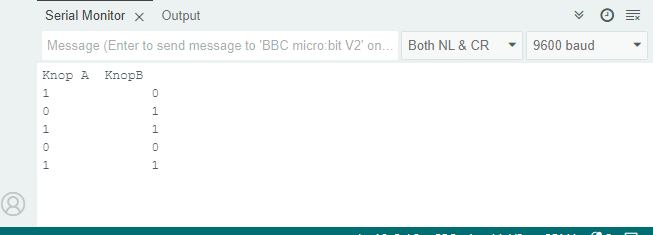
\includegraphics[width=0.6 \linewidth]{figuren/monitorButton}
	\centering
	\caption{Weergave de ingelezen waarde van de bnoppen.}
	\label{fig:button}
\end{figure}
\item De arduino omgeving heeft behalve een \texttt{serial Monitor} ook een \texttt{Serial plotter}. Hierin worden de waarden van de variabele geplot.
De arduino omgeving geeft een korte toelichting op het gebruik van de \href{https://docs.arduino.cc/software/ide-v2/tutorials/ide-v2-serial-plotter/}{serial plotter}. In listing \ref{lst:butplot} zijn twee variabele één variabele heeft altijd de waarde 500, de andere heeft een random waarde.
\begin{lstlisting}[caption={Het uitprinten van een vaste- en een radomwaarde.} ,label={lst:butplot}, numbers=none]
	
int random_variable;
int static_variable = 500;

void setup() {
	Serial.begin(9600);
}

void loop() {
	random_variable = random(0, 1000);
	
	Serial.print("Variable_1:");
	Serial.print(random_variable);
	Serial.print(",");
	Serial.print("Variable_2:");
	Serial.println(static_variable);
	delay(100);
}
	
\end{lstlisting}
Indien deze twee variabel laat uitplotten, wordt iets dergelijks als figuur \ref{fig:plotrnd} weergegeven.
\begin{figure}[H]
	\captionsetup{justification=centering}
	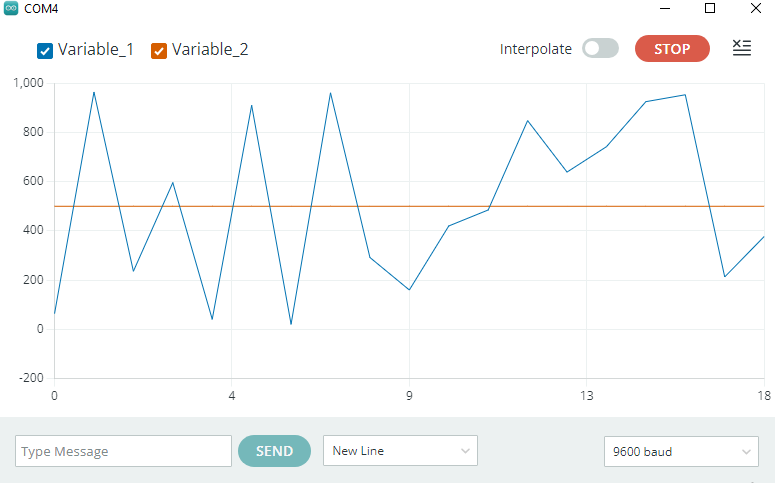
\includegraphics[width=0.7 \linewidth]{figuren/plotVar}
	\centering
	\caption{Het plotten van een vaste en random variabele.}
	\label{fig:plotrnd}
\end{figure}
De \texttt{serial plotter} bepaalt zelf de kleuren van de variabele en de waarde van de Y-as. 
Doordat de waarde van de Y-as bepaald wordt door arduino, kan deze verspringen. Het verspringen van de Y-as kan voorkomen worden door een extra variabele te nemen met een bovengrens, in dit geval is dat 1200.\\
Voeg een bovengrens variabele toe aan listing \ref{lst:butplot} zodat de Y-as gelijk begonnen wordt een maximum van 1200.

\item 
Pas de opdracht van \ref{sec:but} \ref{butNr} zodanig aan zodat op de \texttt{Serial plotter} te zien is wanneer een knop is ingedrukt. Zoals weergegeve in figuur \ref{fig:plotBut}.\\ \textbf{TIP}: Bedenk dat \textit{1 + 2 = 3}.
\begin{figure}[H]
	\captionsetup{justification=centering}
	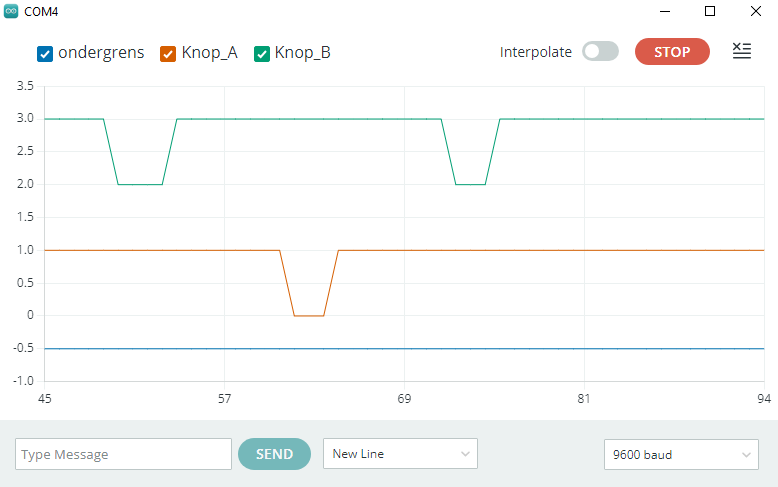
\includegraphics[width=0.8 \linewidth]{figuren/plotBut}
	\centering
	\caption{Het plotten van de stand van de schakelaars met een ondergrens.}
	\label{fig:plotBut}
\end{figure}
\end{enumerate}

\section{Een denderende schakelaar.}

Behalve dat bij het inlezen van de waarde van een externe schakelaar regelmatig een pull\_up weerstand noodzakelijk is. 
Treedt er nog een ander probleem op, namelijk een schakelaar die dendert ook wel bouncing genaamd.

Indien een schakelaar wordt ingedrukt sluit deze bijna nooit in 1 keer, maar veert een aantal keren op en neer. Dit fenomeen wordt weergegeven in Figuur \ref{fig:swDend}, 
\begin{figure}[h!]
	\captionsetup{justification=centering}
	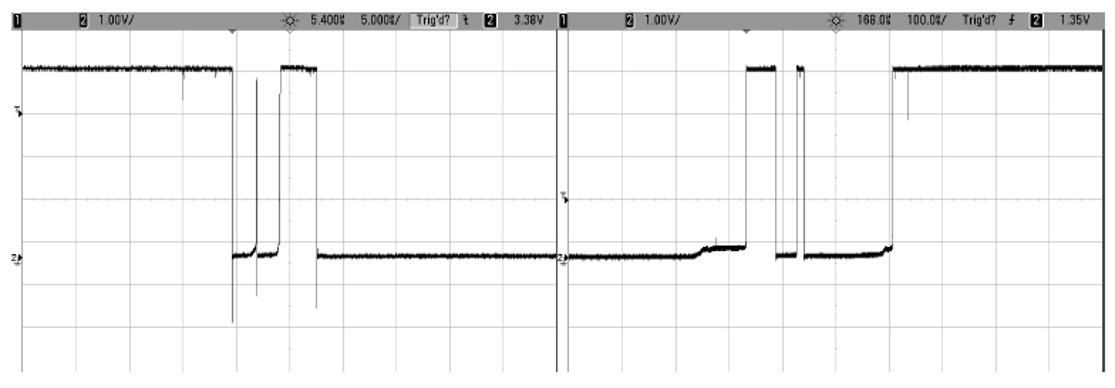
\includegraphics[width=0.6 \linewidth]{figuren/denderen}
	\centering
	\caption{Een denderende schakelaar\cite{williams2014make}.}
	\label{fig:swDend}
\end{figure}
waar te zien is dat bij het indrukken en loslaten van het knopje de schakelaar 'stuitert'. 
Één van de eenvoudigste manieren om dit op te lossen is door even te wachten (een paar milliseconden) en vervolgens te controleren of de knop nog steeds is ingedrukt. Dit wordt weergegeven in listing \ref{lst:denderBut}
%\begin{lstlisting}[style=myArduino, caption= Omgaan met een denderende schakelaar.,label={lst:denderBut}]
\newpage
\begin{lstlisting}[caption= Omgaan met een denderende schakelaar.,label={lst:denderBut}]
	const int knopA = 5;     // Knop A is aangesloten op poortnummer 5
	const int knopB = 11;    // Knop B is aangesloten op poortnummer 11
	
	void setup() {  
		Serial.begin(9600);
		Serial.println("microbit is ready!");
		
		pinMode(knopA, INPUT);  
		pinMode(knopB, INPUT);   
	}
	boolean isKnopIngedrukt(int); //declaratie van de funcie
	
	void loop(){
		
		if( isKnopIngedrukt(knopA) )
		Serial.println("A is ingedrukt");
		
		if( isKnopIngedrukt(knopB) )
		Serial.println("B is ingedrukt");       
		
		delay(10);
	}
	
	boolean isKnopIngedrukt( int knop) {
		if (! digitalRead(knop)) {  //Is de knop soms ingedrukt ?
			delay(2);      //wacht 2 milliseconde 
			if (! digitalRead(knop)) { //Is knop nog steeds ingedrukt
				return true;
			}
		}
		return false;
	}
\end{lstlisting}

Hierbij wordt in de functie \texttt{\textit{\textcolor{arduinoBlue}{boolean} isKnopIngedrukt(\textcolor{arduinoBlue}{int});}} als eerste gekeken of de knop is ingedrukt, vervolgens wordt er 2 milliseconde gewacht, waarna opnieuw gekeken wordt of de knop is ingedrukt. Is dit zo dan wordt een \textcolor{arduinoBlue}{true} mee teruggegeven anders een \textcolor{arduinoBlue}{false}.

In listing \ref{lst:changeBut} is te zien dat er een detectie plaatsvindt wanneer de toestand van de schakelaar verandert.
\begin{lstlisting}[caption= Een toestandverandering van de schakelaar.,label={lst:changeBut}]
	
	const int COL1 = 4; 
	const int ROW1 = 21;
	const int knopA = 5;     // Knop A is aangesloten op poortnummer 5
	const int knopB = 11;    // Knop B is aangesloten op poortnummer 11
	
	boolean isKnopIngedrukt(int);
	
	int knopTeller = 0;  
	boolean knopToestand = false;
	boolean vorigeKnopToestand = false;
	int ledStatus = LOW;
	
	void setup() {  
		Serial.begin(9600);
		Serial.println("microbit is ready!");
		pinMode(COL1, OUTPUT);
		pinMode(ROW1, OUTPUT);
		pinMode(knopA, INPUT);  
		pinMode(knopB, INPUT);   
		digitalWrite(COL1, LOW);
	}
	
	void loop(){
		knopToestand = isKnopIngedrukt(knopA);
		if(knopToestand != vorigeKnopToestand)  //heeft er een verandering plaatsgevonden?
		if (knopToestand == true) {
			knopTeller++;
			ledStatus = !ledStatus;
			Serial.println(knopTeller);
		}
		delay(50);
		vorigeKnopToestand = knopToestand;
		digitalWrite(ROW1, ledStatus);
	}
	
	boolean isKnopIngedrukt( int knop) {
		if (! digitalRead(knop)) {  //Is de knop soms ingedrukt ?
			delay(2);      //wacht 2 milliseconde 
			if (! digitalRead(knop)) { //Is knop nog steeds ingedrukt
				return true;
			}
		}
		return false;
	}
	
\end{lstlisting}

%Open Bestand $\rightarrow$ Voorbeelden $\rightarrow$ Microbit-HHS $\rightarrow$ 04B.StateChangeDetection en
Download    \href{https://github.com/JohnVi-hhs/embsysP/tree/main/voorbeelden/veranderToestandDrukknop.ino}{voorbeeldcode \ref{lst:changeBut} van GitHub} of kopieer listing \ref{lst:changeBut} en upload het naar de Microbit.
Bestudeer de code en kijk hoe het programma werkt. Het is de bedoeling dat na elke druk op knopA de led aan of uit gaat (wisselt van toestand) en dat de teller steeds met 1 opgehoogd wordt. 
\begin{enumerate}[label=(\Alph*)]
	
	\item In figuur \ref{fig:swToestand} wordt het signaal van de button weergegeven.
	\begin{figure}[h!]
		\captionsetup{justification=centering}
		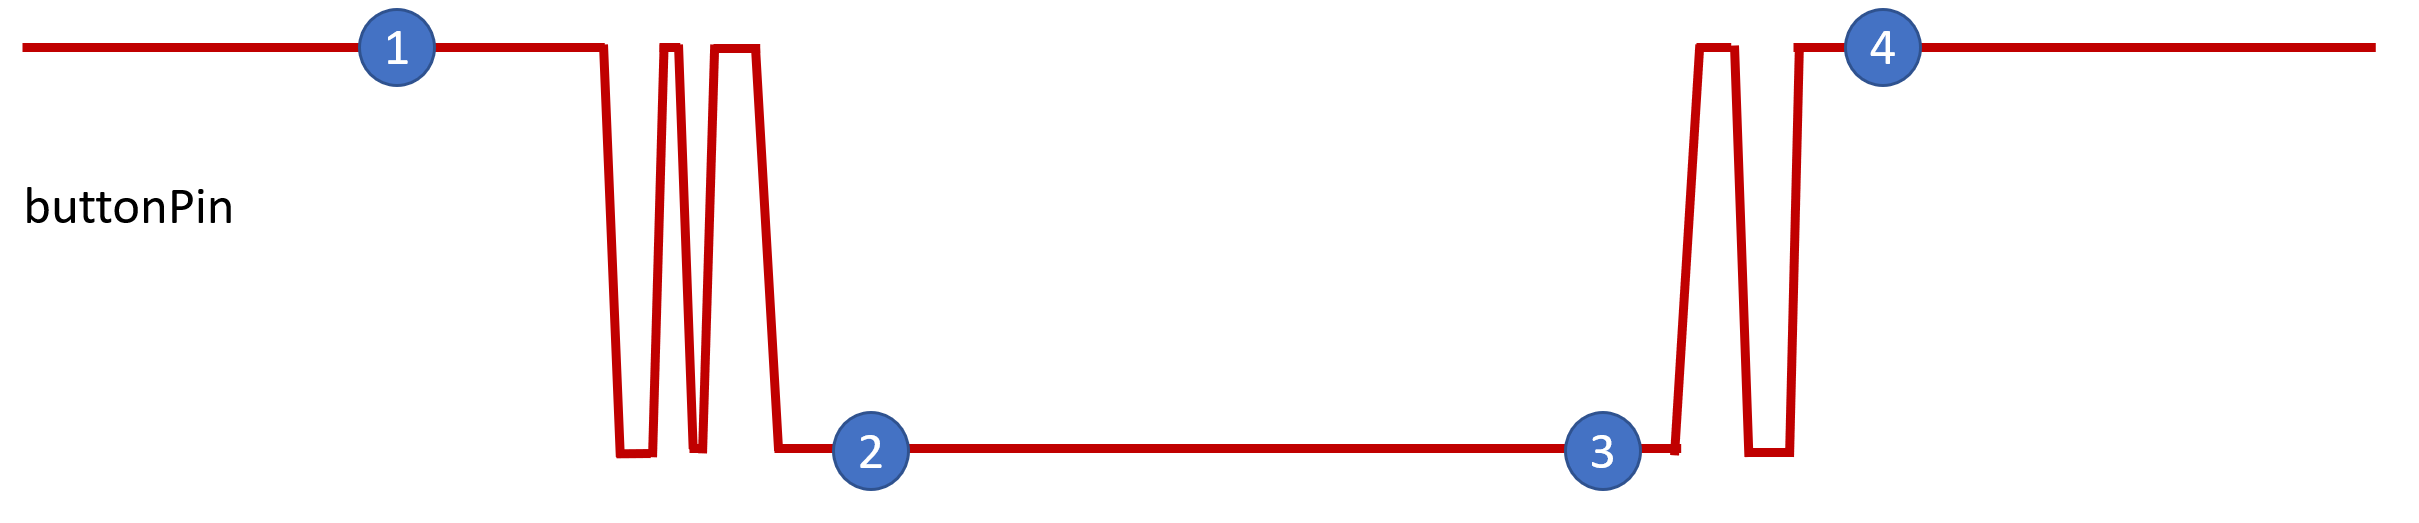
\includegraphics[width=0.8 \linewidth]{figuren/toestandButtonPin}
		\centering
		\caption{Weergaven van het signaal, indien de button wordt ingedrukt en weer wordt losgelaten.}
		\label{fig:swToestand}
	\end{figure}
	In welke toestand (1 t/m 4 )  bevindt zich de variabele \texttt{knopToestand} en \texttt{vorigeKnoptoestand} indien de toestand van de LED verandert en de teller met 1 verhoogd wordt?
	\item Wat is het nut van het statement \textcolor{arduinoOrange}{delay}(50) op regel 31?\hrulefill
	\item Wat is het resultaat indien de outputpin COL1 van listing \ref{lst:changeBut} op \textcolor{arduinoBlue}{HIGH} gezet wordt?	
	\item Breid listing \ref{lst:changeBut} uit, zodat de teller met 1 verlaagd wordt indien met knopB een toestand verandering van 3 naar 4 plaatsvindt.\\
	\textbf{Upload deze opgave op blackboard.}
	
\end{enumerate}

\section{De (externe) pinnen van de microbit}

De Microbit heeft 21 pinnen (aansluitingen) die voor allerlei toepassingen bruikbaar zijn. In figuur \ref{fig:ardPinB} zijn de externe aansluitingen van de microbit te zien. 
\begin{figure}[h!]
	\captionsetup{justification=centering}
	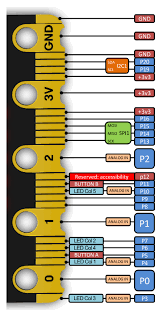
\includegraphics[width=0.4 \linewidth]{figuren/microbitCon}
	\centering
	\caption{Pinlayout van de microbit.}
	\label{fig:ardPinB}
\end{figure}
Hierbij wordt aangegeven welke onderdelen van de microbit ook extern zijn te gebruiken. Bij de pinnen waarbij \fcolorbox{black}{Apricot}{ANALOG IN} staat, kan een externe analoge signaal van b.v. een externe sensor aangesloten worden. De pinnen genaamd \fcolorbox{black}{NavyBlue}{\textcolor{White}{P..}} zijn de pinnummers. In de Arduino IDE kan je die P weglaten en hoef je alleen het nummer op te geven, 0 t/m 20. Uitgebreidere informatie over de pinnen is te vinden op de website \href{https://tech.microbit.org/hardware/edgeconnector/}{tech.microbit.org/hardware/edgeconnector/}.\\
%\newpage

\subsection{Het lezen van externe signalen met de microbit.}

Stel op PIN P0 willen we een externe analoge sensor aansluiten. Voor de spanningswaarde die de sensor levert willen we een digitale waarde weten. 
Dit kan in de Arduino omgeving gedaan worden me het statement:\\

int sensorwaarde = \textcolor{arduinoOrange}{analogRead}(A0);

\begin{enumerate}
	%	\item  Open \textbf{Bestand $\rightarrow$ Voorbeelden $\rightarrow$ 01.Basics $\rightarrow$ AnalogReadSerial}.
	\item In programma listing \ref{lst:analogInp} wordt het analoge signaal van de externe PIN P0 gelezen.
	%\begin{lstlisting}[style=myArduino,numbers=none ,caption= inlezen via een analoog signaal.,label={lst:analogInp}]
	\begin{lstlisting}[numbers=none ,caption= inlezen via een analoog signaal.,label={lst:analogInp}]
		void setup() {  
			pinMode(0, INPUT); 
			Serial.begin(9600);
			Serial.println("Hoi embedded programmeurs!");
		}
		
		void loop(){
			// lees de analoge waarde op pin 0:
			int sensorValue = analogRead(A0);
			
			// print de ingelezen analoge waarde
			Serial.println(sensorValue);
			delay(100);        // delay 
		}
		
	\end{lstlisting}
	\begin{enumerate}
		\item  Maak een nieuw Arduino sketch aan en zet listing \ref{lst:analogInp} erin, Klik vervolgens op \img{figuren/ardIcUpl.png} of druk \colorbox{mygray}{\textbf{Ctrl + U}} om het programma te compileren en naar de Microbit te sturen. 
		\item Zoek PIN 0 in Figuur \ref{fig:ardPinB}.
		\item Leg je Microbit op tafel, raak hem niet aan. 
		\item De Arduino omgeving heeft behalve een Seriële monitor ook een Seriële Plotter. Helaas kan maar één van beide monitor of plotter gebruikt worden. 
		Indien de Seriële monitor open is, sluit deze dan en open de Seriële Plotter ( Tools $\rightarrow$ Serial Plotter of \colorbox{mygray}{\textbf{Ctrl + shift + L}}).
		Raak met je vinger het gouden vlakje van pin 0 aan en kijk in de Seriële Plotter wat er gebeurt.
		\item Tussen welke waardes op de linker as liggen de meetwaardes? \hrulefill \\	
		\footnotesize{\texttt{\textit{(Bij mij kwam deze uit tussen de 1000 zonder aanraken en de 750 )}} }
		
	\end{enumerate}
	
	
	\item Verander he statement  \textcolor{arduinoOrange}{analogRead}(A0); in \textcolor{arduinoOrange}{digitalRead}(A0); Klik vervolgens op \img{figuren/ardIcUpl.png} of druk \colorbox{mygray}{\textbf{Ctrl + U}} om het programma te compileren en naar de Microbit te sturen. Raak met je vinger het gouden vlakje van pin 0 aan en kijk in de Seriële Plotter wat er gebeurt. 
	
	\item Bij het inlezen van een digitaal signaal is het niet wenselijk dat bij het aanraken van een draadje of een gouden vlakje de ingangswaarde instabiel wordt. Om dit te voorkomen kan bij Arduino de  \textcolor{arduinoBlue}{INPUT\_PULLUP} aangezet worden. Dit wordt gedaan met het statement: \textcolor{arduinoOrange}{pinMode}(0,\textcolor{arduinoBlue}{INPUT\_PULLUP}); 
	
	\begin{minipage}{\linewidth}
		\begin{wrapfigure}[25]{r}{0.54\textwidth}
			\vspace{-15pt}
			\begin{center}
				\centering
				\captionsetup{justification=centering}
				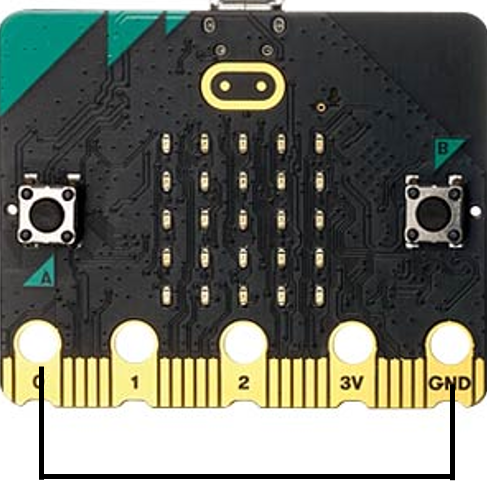
\includegraphics[width=0.32\textwidth]{figuren/microBitDraad}
			\end{center}
			%	\vspace{-14pt}
			\caption{Input verbonden met de GND .}
			\label{fig:micrDraad}
		\end{wrapfigure}
		Zet de \textcolor{arduinoBlue}{INPUT\_PULLUP} aan door het statement 
		\textcolor{arduinoOrange}{pinMode}(0,\textcolor{arduinoBlue}{INPUT\_PULLUP});  
		te plaatsen in de \textcolor{arduinoGreen}{setup} en bekijk wat het resultaat is bij het inlezen van de digitale en analoge waarden. Indien je een draadje bij de hand heb, verbindt de GND met PIN 0, zoals te zien is in figuur \ref{fig:micrDraad}, het gevolg van de PULL\_UP zal zijn dat alleen nog de waarde 0 ingelezen wordt indien de pin ook daadwerkelijk verbonden wordt met de GND.
	\end{minipage}
	
\end{enumerate}

\begin{minipage}{\linewidth}
	\footnotesize{\texttt{\textit{Zoals je ziet is de ingang ongevoelig als je \textcolor{arduinoBlue}{INPUT\_PULLUP} aanzet. Je gebruikt \textcolor{arduinoBlue}{INPUT\_PULLUP} als je een ingang naar een stabiele ‘hoog’ toestand wilt hebben. Je gebruikt deze modus samen met digitalRead() als je een schakelaar wilt uitlezen. Als je de schakelaar indrukt wordt de pin laag.\\
				De knopjes op de Microbit gebruiken een \textbf{externe} pull-up weerstand, met \textcolor{arduinoBlue}{INPUT\_PULLUP} zet je een pull-up weerstand in de microcontroller aan.\\ Kijk eens online voor meer uitleg over de principes van een  \href{https://www.freecodecamp.org/news/a-simple-explanation-of-pull-down-and-pull-up-resistors-660b308f116a/}{pull\_up weerstand}.\\ \\
				Voor verdere uitleg zie \href{https://www.arduino.cc/en/Tutorial/DigitalPins}{www.arduino.cc/en/Tutorial/DigitalPins}
	}}}
\end{minipage}
\normalsize
